\documentclass{article}
\usepackage[utf8]{inputenc}
\usepackage{graphicx}
\graphicspath{ {./images/} }
\usepackage{amsmath}
\usepackage{hyperref}
\usepackage{listings}
\usepackage{csquotes}
\usepackage[english, russian]{babel}

\usepackage[left=2cm,right=1cm, top=2cm,bottom=2cm,bindingoffset=0cm]{geometry}

\renewcommand{\normalsize}{\fontsize{14}{18pt}\selectfont}
\newcommand{\specialcell}[2][c]{%
	\begin{tabular}[#1]{@{}c@{}}#2\end{tabular}}

\renewcommand\refname{Источники}
\title{ Домашнее задание 2    }
\author{ Камилла Файзуллина}
\date{\empty}

\begin{document}
\maketitle
 
 \section{UCSC}
 
  	\begin{table}[h!]
  	\centering
  	\begin{tabular}{|c|c|}
  		\hline
  		имя гена &   OCA2  \\
  		\hline
  	  \specialcell{идентификатор гена \\ в Gencode}  &    ENSG00000104044.16
  	   \\
  		\hline
  		
  		
  		
  		  	  \specialcell{На какой цепи \\ он закодирован}  & Strand: -  \\
  		\hline
  		  	  \specialcell{В какой хромосоме находится}  &  15 \\
  		\hline
  		
  		  	  \specialcell{Плечо и полоса хромосомы}  & \specialcell{ Длиное плечо \\ Полоса 13.1 \\Bands 15q13.1}  \\
  		\hline
  				  	  \specialcell{Cколько альтернативных продуктов}  & 2  \\
  		  	  
  		\hline
  		
  	  		  	  \specialcell{ Транскрипт 1 }  &  
  	  		  	  \specialcell{ 	ENST00000354638.8 \\
  	  		  	  	Chromosome 15: 27,754,875-28,099,315 \\ 24 exons
  	  		  	  	\\838 
    	  	  	} \\
  	\hline
  	
  	  		  	  
  	  		  	  \specialcell{ Транскрипт 2 }  &  
  	  		  	  \specialcell{ENST00000353809.9\\
  	  		  	  Chromosome 15: 27,754,875-28,099,312 \\
  	  		  	  23 exons \\ 814
  	  		  	    } \\
  	\hline	 
  		
  	\end{tabular}
  	\caption{ 1.1 }
  	\label{tab:var}
  \end{table}
  
  \section{Ensembl}
 Процент различий в выравнивании гена OCA2 с гомологичным на 100 нуклеотидов равно примерно $96.4115$. Расхождение нуклеотидов между человеком и шимпанзе по всему геному   в процентах  $1,23$ \cite{compare}. Это досточно схожие значения для выравнивания гена (локального) и полногеномного (глобального). 
   
   
   \section{ Genome Data Viewer}
   В целом, также, как и в других браузерах. Можно понажимать на экзомные участки, также смотреть на них на треках. 
    \begin{figure}[h]
   	\centering
   	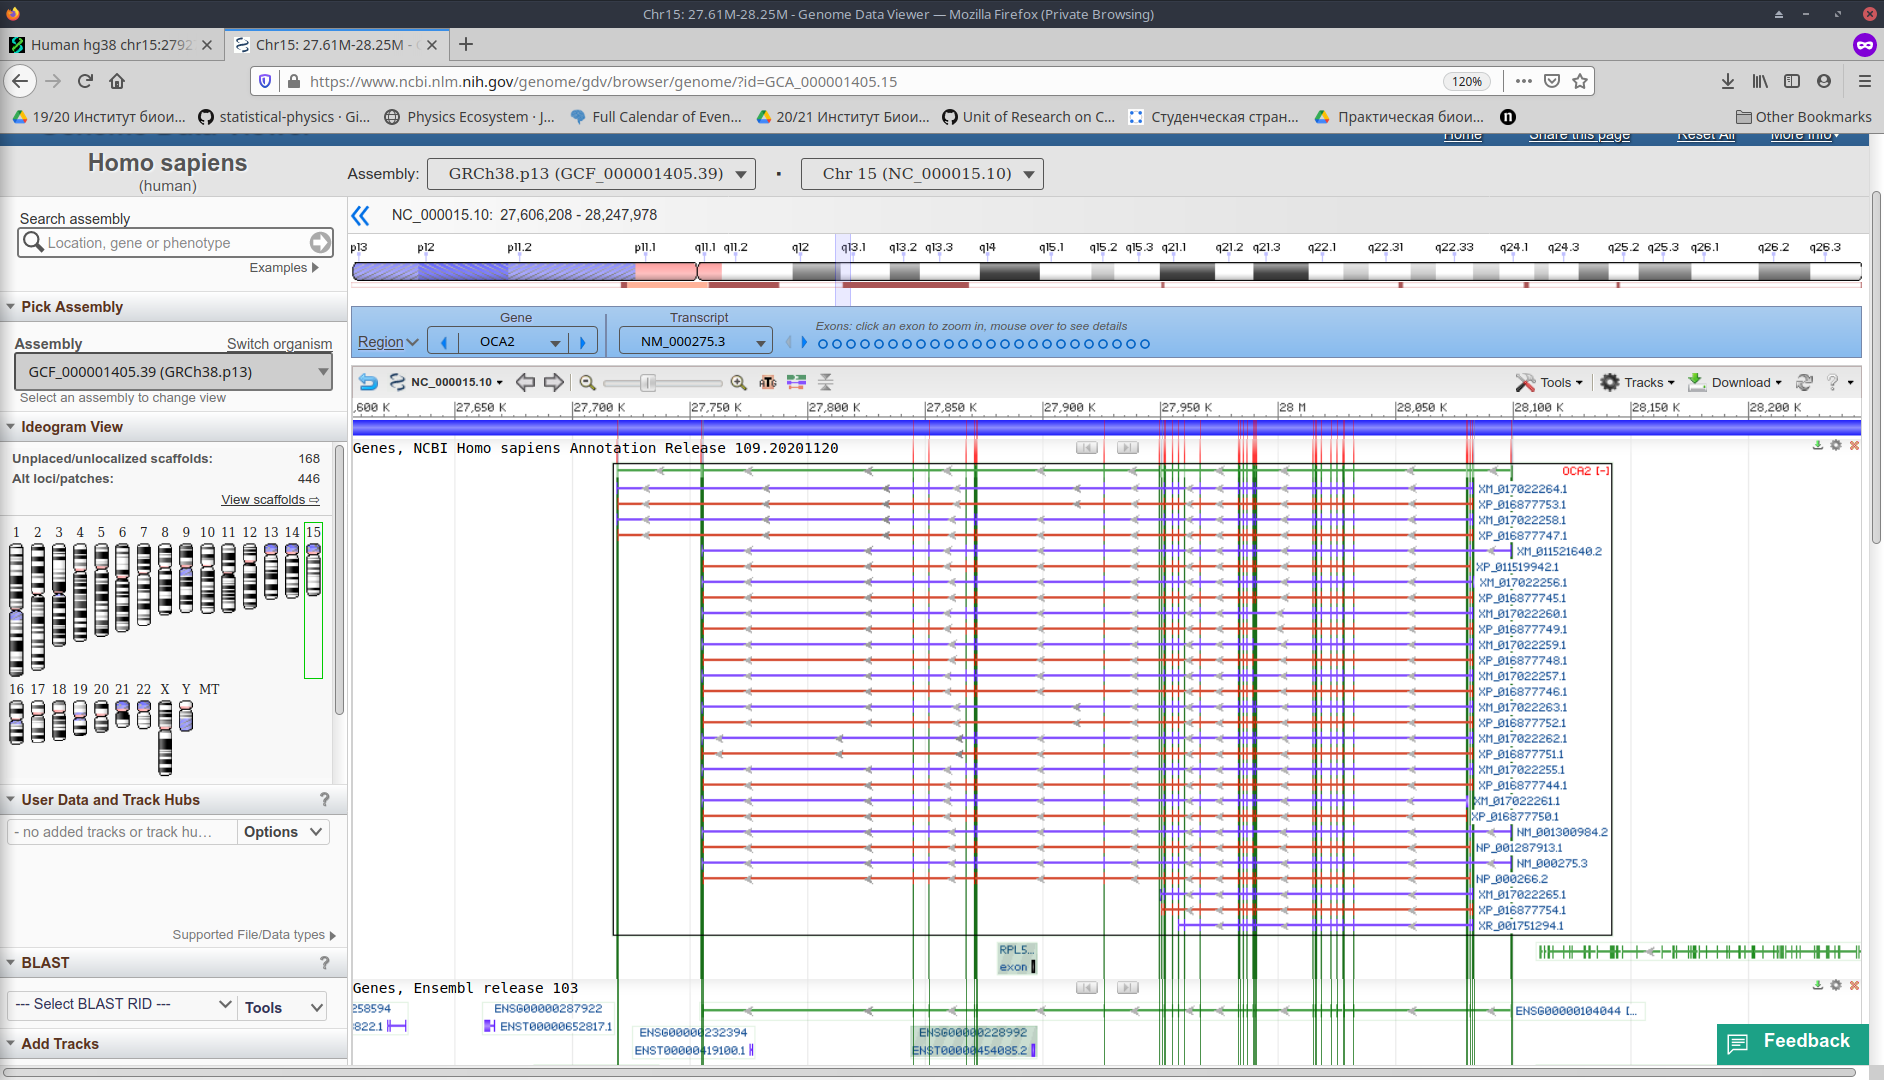
\includegraphics[scale=0.23]{screenncbi}  
   	\caption{ Genome Data Viewer}
   	\label{tree}
   \end{figure}

%\newpage 
%\newpage 
\begin{thebibliography}{9}
 \bibitem{compare}
The Chimpanzee Sequencing and Analysis Consortium., Waterson, R., Lander, E. et al. Initial sequence of the chimpanzee genome and comparison with the human genome. Nature 437, 69–87 (2005). https://doi.org/10.1038/nature04072
\end{thebibliography}




\end{document}